%! TeX program = lualatex
\documentclass[12pt,a4paper]{article}

\usepackage[nil]{babel}
\usepackage{unicode-math}
\usepackage[svgnames]{xcolor}
\usepackage{lmodern}
\usepackage{graphicx}
\usepackage{wrapfig}
\usepackage{float}
\usepackage{parskip}
\usepackage{listings}
\usepackage{adjustbox}

\definecolor{codegreen}{rgb}{0,0.6,0}
\definecolor{codegray}{rgb}{0.5,0.5,0.5}
\definecolor{codepurple}{rgb}{0.58,0,0.82}
\definecolor{backcolour}{rgb}{0.95,0.95,0.92}

\lstdefinestyle{mystyle}{
    backgroundcolor=\color{backcolour},   
    commentstyle=\color{codegreen},
    keywordstyle=\color{magenta},
    numberstyle=\tiny\color{codegray},
    stringstyle=\color{codepurple},
    basicstyle=\ttfamily\footnotesize,
    breakatwhitespace=false,         
    breaklines=true,                 
    captionpos=b,                    
    keepspaces=true,                 
    numbers=left,                    
    numbersep=5pt,                  
    showspaces=false,                
    showstringspaces=false,
    showtabs=false,                  
    tabsize=2
}


\lstset{style=mystyle}

\babelprovide[import=el, main, onchar=ids fonts]{greek} % can also do import=el-polyton
\babelprovide[import, onchar=ids fonts]{english}

\babelfont{rm}
          [Language=Default]{Liberation Sans}
\babelfont[english]{rm}
          [Language=Default]{Liberation Sans}
\babelfont{sf}
          [Language=Default]{Liberation Sans}
\babelfont{tt}
          [Language=Default]{Liberation Sans}

%Enter Title Here
\title{Τεχνολογίες Αποκεντρωμένων Δεδομένων\\Project 2.1: Υλοποίηση Chord}
\author{Γρηγόρης Καπαδούκας (ΑΜ: 1072484)\\Κωνσταντίνος Καπογιάννης (ΑΜ: 1072521)}

\begin{document}
\maketitle
\section{Αρχιτεκτονική Υλοποίησης Εργασίας}
\label{implementation}

\subsection{Προσέγγιση Υλοποίησης}

Στο κεφάλαιο αυτό θα αναλυθούν σημαντικά ζητήματα και σχεδιαστικές αποφάσεις που ακολουθήσαμε κατά την υλοποίησή μας.

\subsubsection{Δημιουργία scraper με σκοπό τη παραγωγή του dataset}

Αρχικά, όπως ζητείται και στην εκφώνηση, έχουμε υλοποιήσει web scraper με σκοπό τη δημιουργία dataset για γνωστούς computer scientists από τη σχετική σελίδα στο Wikipedia.

Επειδή όμως ο σύνδεσμος που δίνει περιέχει μόνο ονόματα και συνδέσμους προς προσωπικές Wikipedia σελίδες, με σκοπό την εύρεση των δεδομένων που ζητούνται ακολουθήσαμε τις εξής προσεγγίσεις:

\begin{itemize}
	\item \textbf{Name:} Αν και η εκφώνηση κανονικά ζητάει μόνο επώνυμο, εμείς αποφασίσαμε πως είναι προτιμότερη η χρήση ονοματεπώνυμου, επειδή πολλοί επιστήμονες στη λίστα έχουν κοινό επώνυμο. Οπότε τα ονοματεπώνυμα τα βρίσκουμε στον αρχικό σύνδεσμο που μας δόθηκε.
	\item \textbf{Awards:} Με σκοπό την εύρεση του αριθμού βραβείων φορτώνουμε αρχικά φορτώνουμε τη προσωπική σελίδα του επιστήμονα από σύνδεσμο που βρίσκεται στην αρχική σελίδα της λίστας επιστημόνων. Έπειτα ψάχνουμε στη προσωπική σελίδα για παράγραφο με τίτλο που περιέχει τη λέξη 'Awards'. Παρατηρούμε πως στις σελίδες των επιστημόνων συνηθίζεται να αναφέρονται ονομαστικά όλα τα awards σε πολλά bullets.

	      Οπότε αποφασίσαμε για να εξάγουμε τον αριθμό των awards να μετρήσουμε απλά τον αριθμό των bullets και να αποθηκεύσουμε στο παραγόμενο dataset τον αντίστοιχο αριθμό για κάθε επιστήμονα.

	      Σημειώνουμε εδώ πως δεν αναφέρονται σε όλες τις προσωπικές σελίδες τα awards του επιστήμονα, οπότε στη περίπτωση που αυτά δεν βρεθούν αποθηκεύουμε τη τιμή NaN.
	\item \textbf{Institution:} Εδώ αρχικά αναφέρουμε ότι αποθηκεύουμε τα Institutions με τα οποία είναι συσχετισμένος ο επιστήμονας, αντί για 'Education' όπως ζητείται, επειδή για πολλούς επιστήμονες υπάρχει μόνο πληροφορία για εταιρίες που δούλεψαν (πχ AT\&T) οπότε θέλουμε να υποστηρίξουμε queries και για αυτούς.

	      Οπότε για να βρούμε τη πληροφορία που χρειαζόμαστε βρίσκουμε στη προσωπική σελίδα του επιστήμονα κάθε φορά το πεδίο 'Institutions' στο προσωπικό side card, από όπου αποθηκεύουμε όλα τα institutions που εμφανίζονται.
\end{itemize}

Σημειώνουμε εδώ πως το τελικό dataset το αποθηκεύουμε σε μορφή CSV, όπου όμως για κάθε επιστήμονα που είναι συσχετισμένος με πολλά institutions γίνονται πολλαπλές εισαγωγές, μια για κάθε institution. Με αυτό το τρόπο μπορούμε εύκολα μετέπειτα μέσω κώδικα να κάνουμε group τα δεδομένα με βάση το institution και να εισάγουμε τα groupings στους Chord κόμβους.

Το dataset το παρέχουμε στην υποβολή της εργασίας με το όνομα\\'list\_of\_computer\_scientists.csv'.

\subsubsection{Σχεδιαστικές Λεπτομέρειες της Chord Υλοποίησης}

Με σκοπό την εξήγηση της Chord υλοποίησής μας, αναφέρω αρχικά πως έχουμε ακολουθήσει προσέγγιση με multiprocessing για να κάνουμε spawn τους κόμβους. Οπότε κάθε κόμβος δημιουργείται ως μια ξεχωριστή διεργασία του λειτουργικού συστήματος.

Επειδή όμως οι διεργασίες δεν έχουν κοινή μνήμη, αυτό δημιουργεί την ανάγκη για σύστημα επικοινωνίας μεταξύ των κόμβων. Για την επικοινωνία λοιπόν χρησιμοποιούμε sockets ώστε μέσω TCP να μπορούν να στέλνονται οι αναγκαίες πληροφορίες μεταξύ των κόμβων.

Τέλος, με σκοπό το concurrent handling της αναμονής για συνδέσεις από άλλους κόμβους, της εκτέλεσης του stabilize routine, την εκτέλεση της fix fingers routine και τον έλεγχο ότι οι successors του successor list είναι ακόμα online έχουμε χρησιμοποιήσει multithreading. Οπότε κάθε κόμβος, που αποτελεί ένα process, έχει επίσης τέσσερα threads, ένα για κάθε λειτουργία που αναφέρθηκε παραπάνω.

Οπότε με τη προσέγγιση αυτή επιτυγχάνουμε να σχεδιάσουμε μια υλοποίηση του πρωτοκόλλου του Chord που είναι πραγματικά αποκεντρωμένη, εφόσον όχι μόνο εκτελούνται όλοι οι κόμβοι σε διαφορετικές διεργασίες, αλλά ταυτόχρονα εφόσον γίνεται η επικοινωνία με sockets θα μπορούσε να γίνει deployed σε πολλά μηχανήματα σε διάφορες γεωγραφικές περιοχές.

Προτιμήσαμε αυτή τη προσέγγιση επειδή οι μετρήσεις που θα κάνουμε στο τέλος της εργασίας θα αντιπροσωπεύουν καλύτερα αυτό που θα βλέπαμε σε πραγματική χρήση του πρωτοκόλλου, σε σχέση με άλλες μη παραλληλοποιημένες υλοποιήσεις, εφόσον έχουμε κάνει μια πραγματική αποκεντωμένη υλοποίηση.

\subsection{Περιβάλλον Υλοποίησης Εργασίας}

Η εργασία έχει υλοποιηθεί σε γλώσσα προγραμματισμού Python. Οι πιο αξιοσημείωτες βιβλιοθήκες που έχουν χρησιμοποιηθεί είναι οι εξής:

\begin{itemize}
	\item \textbf{httpx:} Χρήση στο scraper για να γίνουν GET requests στη Wikipedia στο Python κώδικα.
	\item \textbf{BeautifulSoup:} Χρήση στο scraper με σκοπό τον χειρισμό των απαντήσεων της Wikipedia στα ερωτήματα του httpx, και την απομόνωση και το χειρισμό της χρήσιμης πληροφορίας για τη παραγωγή του dataset.
	\item \textbf{hashlib:} Χρησιμοποιείται για την παραγωγή των IDs των κόμβων και των δεδομένων για την εισαγωγή τους αντίστοιχα στο δίκτυο Chord, καθώς και στα lookups όταν θέλουμε να παράγουμε από ερωτήματα τα IDs που θα ψάξουμε.
	\item \textbf{multiprocessing:} Χρησιμοποιείται για τη δημιουργία πολλών Chord κόμβων στο ίδιο σύστημα, όπου ο καθένας αποτελεί μια διεργασία.
	\item \textbf{pandas:} Χρησιμοποιείται για την αποθήκευση και το χειρισμό του dataset που παράγουμε μέσω του scraper, ως CSV αρχείο.
	\item \textbf{pickle:} Χρησιμοποιείται για να σταλθούν ολόκληρες μεταβλητές μεταξύ κόμβων μέσω sockets. Οπότε ο αποστολέας κάνει dump το περιεχόμενο της μεταβλητής σε pickle object, το οποίο μπορεί να σταλθεί μέσω του socket και να το κάνει load ο παραλήπτης σε δική του μεταβλητή.
	\item \textbf{socket:} Χρησιμοποιείται για την επικοινωνία μεταξύ κόμβων.
	\item \textbf{threading:} Χρησιμοποιείται ώστε κάθε κόμβος να είναι multithreaded, ώστε να μπορεί να δέχεται ερωτήματα από άλλους, να τρέχει τη stabilize routine, να κάνει update fingers και να ελέγχει τον immediate successor list όλα concurrently.
\end{itemize}

Σημειώνουμε ότι για την εγκατάσταση των βιβλιοθηκών σε virtual environment, έχουμε χρησιμοποιήσει το εργαλείο Miniconda (το Anaconda λειτουργεί με ακριβώς τον ίδιο τρόπο). Έχουμε συμπεριλάβει το αρχείο environment.yml που μπορεί να χρησιμοποιηθεί για να δημιουργηθεί πανομοιότυπο environment με το δικό μας περιβάλλον υλοποίησης, με σκοπό την εκτέλεση του κώδικα.

\subsection{Οδηγίες Εκτέλεσης Κώδικα}

\begin{enumerate}
	\item Αρχικά εγκαταστήστε το Miniconda (ή το Anaconda) ώστε να μπορέσετε μέσω αυτού να δημιουργήσετε virtual environment με τις απαραίτητες βιβλιοθήκες.
	\item Εκτελέστε τις παρακάτω εντολές για να δημιουργήσετε και ενεργοποιήσετε το virtual environment:
	      \begin{lstlisting}[language=Bash, breaklines=true, tabsize=2, basicstyle=\footnotesize]
conda env create -f environment.yml
conda activate dd\end{lstlisting}
	\item Έπειτα παραμετροποιήστε τις εξής υπερπαραμέτρους στο αρχείο\\main.py
	      \begin{itemize}
		      \item \textbf{num\_nodes:} Ο αριθμός των κόμβων (άρα και διεργασιών) που θα δημιουργηθούν.
		      \item \textbf{size\_successor\_list:} Το μέγεθος του successor list κάθε κόμβου.
		      \item \textbf{base\_port:} Το port number στο οποίο θα ακούει για επικοινωνία ο πρώτος κόμβος (οι υπόλοιποι ακούνε σε port numbers +1 κάθε φόρα, πχ για 40 κόμβους με base\_port 8000 θα δεσμευτούν τα ports 8000 μέχρι 8039)
		      \item \textbf{stabilize\_interval:} Η συχνότητα σε δευτερόλεπτα που εκτελείται η stabilize routine κάθε κόμβου.
		      \item \textbf{fix\_fingers\_interval:} Η συχνότητα σε δευτερόλεπτα που εκτελείται η fix fingers routine κάθε κόμβου.
		      \item \textbf{ping\_successors\_inverval:} Η συχνότητα σε δευτερόλεπτα\\που κάθε κόμβος επικοινωνεί με τους successors στο successor list με σκοπό να εντοπίσει αν κάποιος έφυγε και να διατηρήσει τον immediate successor. Το successor list επίσης διορθώνεται από το stabilize routine στη περίπτωση νέων εισαγωγών.
	      \end{itemize}
	\item Μετά, εκτελέστε τον κώδικα με την εξής εντολή:
	      \begin{lstlisting}[language=Bash, breaklines=true, tabsize=2, basicstyle=\footnotesize]
python main.py\end{lstlisting}
	\item Τέλος εφόσον βρεθείτε στο console, ακολουθήστε τις οδηγίες που εμφανίζονται για να κάνετε ερωτήματα στους κόμβους.

	      Σημειώνω επίσης πως το console επιτρέπει απλά τη σύνδεση και τα ερωτήματα στους κόμβους που δημιουργήθηκαν μέσω επικοινωνίας με sockets. Οπότε όλες οι εντολές που στέλνονται μεταξύ κόμβων, μπορούν να σταλθούν και μέσω του console, με εξαίρεση αυτών που στέλνουν μεταβλητές μέσω pickle.

	      Για πλήρη λίστα εντολών μπορείτε να ανατρέξετε στο κώδικα του chord.py στη handle\_commands μέθοδο.
\end{enumerate}

\subsection{Screenshots Εκτέλεσης του Κώδικα}

Παρακάτω δίνω ένα παράδειγμα εκτέλεσης του κώδικα για 40 κόμβους και ερώτημα στο πρώτο για ένα βασικό lookup.
\begin{figure}[H]
	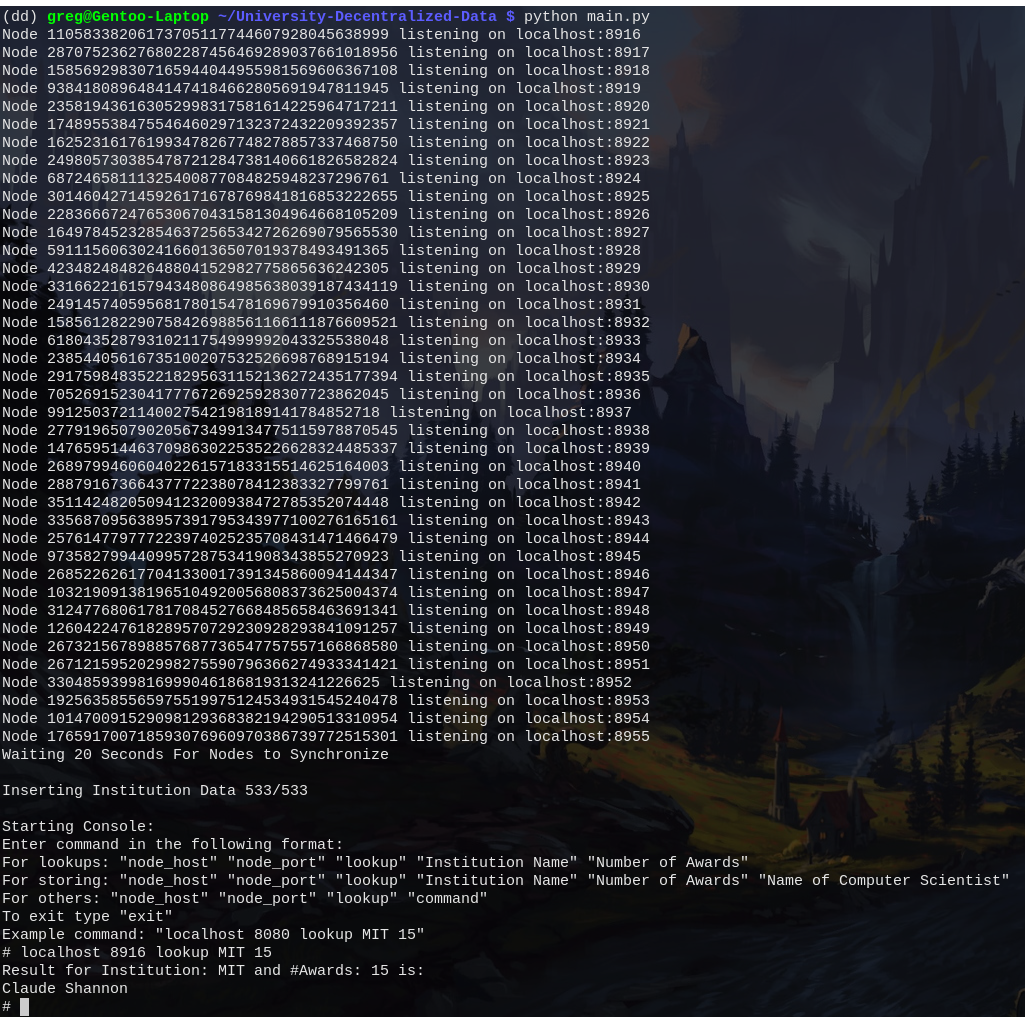
\includegraphics[width=\textwidth]{images/code_execution_example.png}
	\caption{Παράδειγμα Εκτέλεσης Κώδικα}
	\label{code_execution_example}
\end{figure}

\section{Πειραματική Αξιολόγηση των Βασικών Πράξεων}

\subsection{Εξήγηση Πειραματικής Προσέγγισης}
\label{experimental_methodology}

Λόγω της προσέγγισης υλοποίησης που επιλέξαμε που εξηγήθηκε στο κεφάλαιο \ref{implementation}, προσεγγίζουμε την πειραματική αξιολόγηση με ιδιαίτερο τρόπο. Αυτό συμβαίνει επειδή το δίκτυο είναι πραγματικά αποκεντρωμένο και δεν είναι στο spec του πρωτοκόλλου να μελετάται πληροφορία όπως ο αριθμός των hops (σε lookup) ή ο χρόνος που απαιτείται για να εκτελεστεί κάποια βασική πράξη.

Οπότε με σκοπό να αξιολογήσουμε πειραματικά την υλοποίησή μας χρησιμοποιούμε αντίστοιχα print statements με σκοπό να μετρήσουμε τον αριθμό μηνυμάτων που στέλνονται (τα οποία δίνονται αρχικά commented στην τελική έκδοση της υποβολής). Άρα έτσι μπορούμε να εξάγουμε τη πληροφορία που θέλουμε στο stdout χωρίς να αλλάξουμε δραστικά το πρωτόκολλο με τρόπους που θα μπορούσε να επηρεάσει τις μετρικές (πχ να συγχρονίζαμε τους κόμβους μετά από join για να δούμε πόσο χρόνο θα πάρει είναι χρονοβόρο και καταστρέφει τη ποιότητα του αποτελέσματος).

Άρα αποφασίσαμε να μετρήσουμε τον αριθμό των μηνυμάτων μεταξύ όλων των κόμβων κατά τη διάρκεια κάποιου operation. Αυτό θα οδηγήσει σε μεγάλο αριθμό μηνυμάτων, όπως θα δούμε παρακάτω, αλλά αυτό είναι αναμενόμενο, εφόσον προσμετρούνται και μηνύματα που στέλνονται από κόμβους άσχετα με τη λειτουργία που μελετάμε, αλλά για τη διατήρηση του δικτύου (πχ stabilize, fix fingers και ping successor list). Παρόλα αυτά θέλουμε ακόμα να επικυρώσουμε το scaling των operations όπως τα υπολόγισαν οι ερευνητές που εισήγαγαν το Chord, δηλαδή $O(logN)$ μηνύματα για lookup και $O(log^2Ν)$ μηνύματα για join και leave. Ταυτόχρονα θα δούμε σε μια πραγματική υλοποίηση πόσα μηνύματα στέλνονται κατά τη διάρκεια των operations, για να επιτευχθούν και ταυτόχρονα να διατηρηθεί το δίκτυο.

Σημειώνουμε επίσης πως θεωρούμε το χρόνο που παίρνει το lookup, join και leave ασήμαντη πληροφορία, εφόσον τα αποκεντρωμένα δίκτυα χαρακτηρίζονται από ανομοιογένεια υπολογιστικών πόρους στους κόμβους, και από μεγάλες γεωγραφικές εκτάσεις απόστασης που μπορούν να προσθέσουν latency, άρα αν μελετούσαμε πειραματικό χρόνο τα αποτελέσματα θα ήταν ασήμαντα για σύγκριση με τη περίπτωση του deployment της εφαρμογής.

Τέλος σημειώνω πως κρατάμε τον αριθμό των κόμβων σχετικά χαμηλό στα πειράματά μας, λόγω περιορισμού υπολογιστικών πόρων (εφόσον κάθε κόμβος είναι διεργασία με 4 threads, άρα πχ για 40 κόμβους έχουμε 40 διεργασίες και 160 threads).

\subsection{Πειραματικά Αποτελέσματα}

Αποφασίσαμε να κάνουμε πειραματικές μετρήσεις για αριθμούς κόμβων ίσο με 20, 30, 40 και 50. Προφανώς κάνουμε τις μετρήσεις κάνοντας το operation πάνω σε ένα ήδη αρχικοποιημένο δίκτυο με τον αριθμό κόμβων που αναφέρεται κάθε φορά.

Επίσης παίρνουμε το μέσο όρο μηνυμάτων που στάλθηκαν για 10 εκτελέσεις για κάθε περίπτωση, εφόσον η τυχαιότητα στη κατάσταση του χρονομέτρου που εκτελεί το stabilize, το fix fingers και το ping successors τη στιγμή που γίνεται το operation καθώς και το hash space μπορεί να επηρεάσει τα αποτελέσματα.

Οι υπερπαράμετροι που ορίσαμε για τα πειράματά μας είναι οι εξής:
\begin{itemize}
	\item size\_successor\_list = 5
	\item stabilize\_interval = 0.5
	\item fix\_fingers\_interval = 0.3
	\item ping\_successors\_interval = 0.2
\end{itemize}

Στο πίνακα \ref{resuls_table}, δίνουμε τα πειραματικά αποτελέσματα μας για κάθε περίπτωση αριθμού κόμβων προς το μέσο αριθμό μηνυμάτων και τη διασπορά για κάθε μια από τις βασικές πράξεις:

\begin{table}[H]
	\centering
	\begin{adjustbox}{width={0.8\textwidth},totalheight={0.8\textheight},keepaspectratio}%
		\begin{tabular}{|c|c|c|}
			\hline
			\textbf{Πράξη - Αριθμός Κόμβων} & \textbf{Μέση Τιμή} & \textbf{Διασπορά} \\
			\hline
			Join - 20                       & 291.4              & 14558.4888        \\
			\hline
			Join - 30                       & 454.5              & 22880.2777        \\
			\hline
			Join - 40                       & 702.1              & 53607.4333        \\
			\hline
			Join - 50                       & 541.1              & 38822.5444        \\
			\hline
			Leave - 20                      & 605.8              & 161341.2888       \\
			\hline
			Leave - 30                      & 1027.3             & 263307.5666       \\
			\hline
			Leave - 40                      & 1410.1             & 602828.9888       \\
			\hline
			Leave - 50                      & 1479.1             & 706898.1          \\
			\hline
			Lookup - 20                     & 8703.3             & 98150.9           \\
			\hline
			Lookup - 30                     & 13575.8            & 129595.5111       \\
			\hline
			Lookup - 40                     & 26338.9            & 397592082.9888    \\
			\hline
			Lookup - 50                     & 23339.8            & 790500.6222       \\
			\hline
		\end{tabular}
	\end{adjustbox}
	\caption{Πίνακας Πειραματικών Αποτελεσμάτων}
	\label{resuls_table}
\end{table}

Επίσης στα σχήματα \ref{join_figure}, \ref{leave_figure}, \ref{lookup_figure}, \ref{all_figure} δίνουμε γραφικές παραστάσεις της μέσης τιμής μηνυμάτων για τις πράξεις join, leave, lookup και όλες συνδυαστικά αντίστοιχα.

\begin{figure}[H]
	\centering
	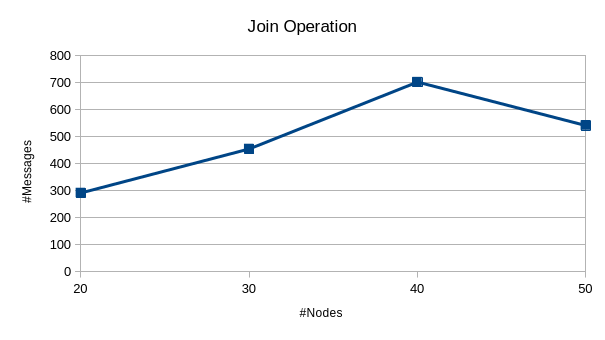
\includegraphics[scale=0.55]{./images/join.png}
	\caption{Σχήμα για Join}
	\label{join_figure}
\end{figure}

\begin{figure}[H]
	\centering
	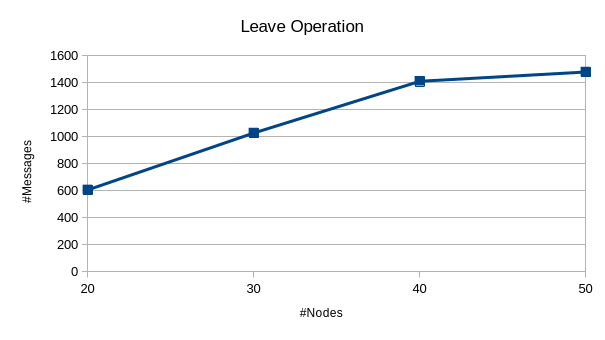
\includegraphics[scale=0.55]{./images/leave.png}
	\caption{Σχήμα για Leave}
	\label{leave_figure}
\end{figure}

\begin{figure}[H]
	\centering
	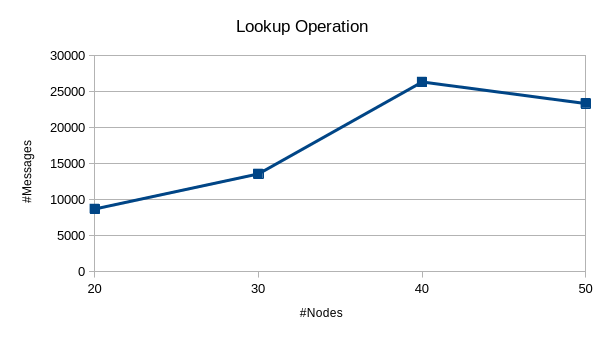
\includegraphics[scale=0.55]{./images/lookup.png}
	\caption{Σχήμα για Lookup}
	\label{lookup_figure}
\end{figure}

\begin{figure}[H]
	\centering
	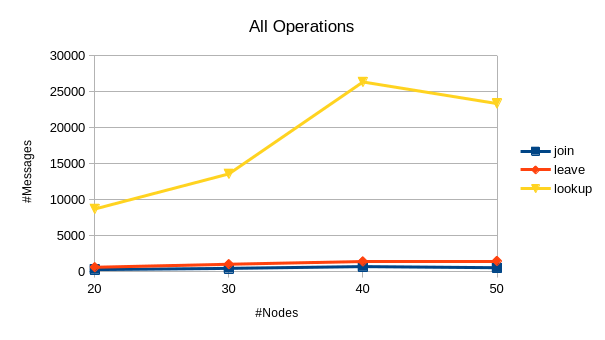
\includegraphics[scale=0.6]{./images/all.png}
	\caption{Σχήμα για όλες τις πράξεις}
	\label{all_figure}
\end{figure}

Σημειώνουμε πως έχουμε συμπεριλάβει ένα excel αρχείο όπου υπολογίσαμε τους μέσους όρους και τις διασπορές και φτιάξαμε τα γραφήματα, καθώς και αρχεία με το output των benchmarks που χρησιμοποιήσαμε για να μετρήσουμε τα μηνύματα που στάλθηκαν στο φάκελο 'benchmarks'.

\subsection{Ερμηνεία Αποτελεσμάτων}

\textbf{Σημείωση:} Αρχικά αναφέρουμε ξανά, πως ο λόγος που τα μηνύματα που στέλνονται είναι τόσο πολλά είναι επειδή όπως εξηγήσαμε στο κεφάλαιο \ref{experimental_methodology}, μετράμε όχι μόνο τα σχετικά μηνύματα για τις πράξεις αλλά και όλα τα υπόλοιπα μηνύματα που στέλνονται μέσα στο δίκτυο. Ο λόγος που ακολουθήσαμε αυτή τη προσέγγιση εξηγήθηκε επίσης στο κεφάλαιο \ref{experimental_methodology}.

Αναφέρουμε ξανά πως σύμφωνα με το paper του Chord ο αριθμός των μηνυμάτων που στέλνεται για join και leave operations είναι $O(log^2N)$ και για lookup operations είναι $O(logN)$. Από τα σχήματα \ref{join_figure}, \ref{leave_figure}, \ref{lookup_figure} και \ref{all_figure} παρατηρούμε πως όντως τα πειραματικά μας αποτελέσματα επικυρώνουν αυτά τα scaling factors.

Παρόλα αυτά παρατηρούμε πως για 50 κόμβους στο join και στο lookup τα μηνύματα είναι λιγότερα από τη περίπτωση των 40 κόμβων. Αυτό πιθανότατα προκύπτει τυχαία από το σχετικά μικρό αριθμό εκτελέσεων, εφόσον παρατηρούμε πως και οι τιμές της διασποράς γενικά είναι υψηλές.

Οπότε συμπεραίνουμε πως με τα πειραματικά αποτελέσματά μας επικυρώσαμε ότι η υλοποίηση ακολουθεί την απαίτηση μηνυμάτων όπως αναφέρεται στο paper του Chord, καθώς και παρατηρήσαμε τον αριθμό μηνυμάτων που θα μπορούσε να έχει ένα τέτοιο δίκτυο σε μια πραγματική υλοποίηση.

\end{document}
